\documentclass[]{book}
\usepackage{lmodern}
\usepackage{amssymb,amsmath}
\usepackage{ifxetex,ifluatex}
\usepackage{fixltx2e} % provides \textsubscript
\ifnum 0\ifxetex 1\fi\ifluatex 1\fi=0 % if pdftex
  \usepackage[T1]{fontenc}
  \usepackage[utf8]{inputenc}
\else % if luatex or xelatex
  \ifxetex
    \usepackage{mathspec}
  \else
    \usepackage{fontspec}
  \fi
  \defaultfontfeatures{Ligatures=TeX,Scale=MatchLowercase}
\fi
% use upquote if available, for straight quotes in verbatim environments
\IfFileExists{upquote.sty}{\usepackage{upquote}}{}
% use microtype if available
\IfFileExists{microtype.sty}{%
\usepackage{microtype}
\UseMicrotypeSet[protrusion]{basicmath} % disable protrusion for tt fonts
}{}
\usepackage[margin=1in]{geometry}
\usepackage{hyperref}
\hypersetup{unicode=true,
            pdftitle={Applied Time Series Analysis},
            pdfauthor={Vipul Bhatt},
            pdfborder={0 0 0},
            breaklinks=true}
\urlstyle{same}  % don't use monospace font for urls
\usepackage{natbib}
\bibliographystyle{apalike}
\usepackage{longtable,booktabs}
\usepackage{graphicx,grffile}
\makeatletter
\def\maxwidth{\ifdim\Gin@nat@width>\linewidth\linewidth\else\Gin@nat@width\fi}
\def\maxheight{\ifdim\Gin@nat@height>\textheight\textheight\else\Gin@nat@height\fi}
\makeatother
% Scale images if necessary, so that they will not overflow the page
% margins by default, and it is still possible to overwrite the defaults
% using explicit options in \includegraphics[width, height, ...]{}
\setkeys{Gin}{width=\maxwidth,height=\maxheight,keepaspectratio}
\IfFileExists{parskip.sty}{%
\usepackage{parskip}
}{% else
\setlength{\parindent}{0pt}
\setlength{\parskip}{6pt plus 2pt minus 1pt}
}
\setlength{\emergencystretch}{3em}  % prevent overfull lines
\providecommand{\tightlist}{%
  \setlength{\itemsep}{0pt}\setlength{\parskip}{0pt}}
\setcounter{secnumdepth}{5}
% Redefines (sub)paragraphs to behave more like sections
\ifx\paragraph\undefined\else
\let\oldparagraph\paragraph
\renewcommand{\paragraph}[1]{\oldparagraph{#1}\mbox{}}
\fi
\ifx\subparagraph\undefined\else
\let\oldsubparagraph\subparagraph
\renewcommand{\subparagraph}[1]{\oldsubparagraph{#1}\mbox{}}
\fi

%%% Use protect on footnotes to avoid problems with footnotes in titles
\let\rmarkdownfootnote\footnote%
\def\footnote{\protect\rmarkdownfootnote}

%%% Change title format to be more compact
\usepackage{titling}

% Create subtitle command for use in maketitle
\newcommand{\subtitle}[1]{
  \posttitle{
    \begin{center}\large#1\end{center}
    }
}

\setlength{\droptitle}{-2em}

  \title{Applied Time Series Analysis}
    \pretitle{\vspace{\droptitle}\centering\huge}
  \posttitle{\par}
    \author{Vipul Bhatt}
    \preauthor{\centering\large\emph}
  \postauthor{\par}
      \predate{\centering\large\emph}
  \postdate{\par}
    \date{2018-09-19}

\usepackage{booktabs}
\usepackage{amsthm}
\makeatletter
\def\thm@space@setup{%
  \thm@preskip=8pt plus 2pt minus 4pt
  \thm@postskip=\thm@preskip
}
\makeatother

\usepackage{amsthm}
\newtheorem{theorem}{Theorem}[chapter]
\newtheorem{lemma}{Lemma}[chapter]
\theoremstyle{definition}
\newtheorem{definition}{Definition}[chapter]
\newtheorem{corollary}{Corollary}[chapter]
\newtheorem{proposition}{Proposition}[chapter]
\theoremstyle{definition}
\newtheorem{example}{Example}[chapter]
\theoremstyle{definition}
\newtheorem{exercise}{Exercise}[chapter]
\theoremstyle{remark}
\newtheorem*{remark}{Remark}
\newtheorem*{solution}{Solution}
\let\BeginKnitrBlock\begin \let\EndKnitrBlock\end
\begin{document}
\maketitle

{
\setcounter{tocdepth}{1}
\tableofcontents
}
\hypertarget{preface}{%
\chapter*{Preface}\label{preface}}
\addcontentsline{toc}{chapter}{Preface}

These lecture notes are prepared for an upper level undergraduate course
in time series econometrics. Every fall I teach a course on applied time
series analysis at James Madison University. These notes borrow heavily
from the teaching material that I have developed over several years of
instruction of this course.

One of my main objective is to develop a primer on time series analysis
that is more accessible to undergraduate students than standard
textbooks available in the market. Most of these textbooks in my opinion
are densely written and assume advanced mathematical skills on the part
of our students. Further, I have also struggled with their topic
selection and organization. Often I end up not following the chapters in
order and modify content (by adding or subtracting) to meet my students
needs. Such changes causes confusion for some students and more
importantly discourages optimal use of the textbook. Hence, this is an
undertaking to develop a primer on time series that is accessible,
follows a more logical sequencing of topics, and covers content that is
most useful for undergraduate students in business and economics.

\emph{Note: These notes have been prepared by me using various sources,
published and unpublished. All errors that remain are mine.}

\hypertarget{intro}{%
\chapter{Introduction to Forecasting}\label{intro}}

\hypertarget{time-series}{%
\section{Time Series}\label{time-series}}

A time series is a specific kind of data where observations of a
variable are recorded over time. For example, the data for the U.S. GDP
for the last 30 years is a time series data.

Such data shows how a variable is changing over time. Depending on the
variable of interest we can have data measured at different frequencies.
Some commonly used frequencies are intra-day, daily, weekly, monthly,
quarterly, semi-annual and annual. Figure \ref{fig:ch1-figure1} below
plots data for quarterly and monthly frequency.

\begin{figure}

{\centering 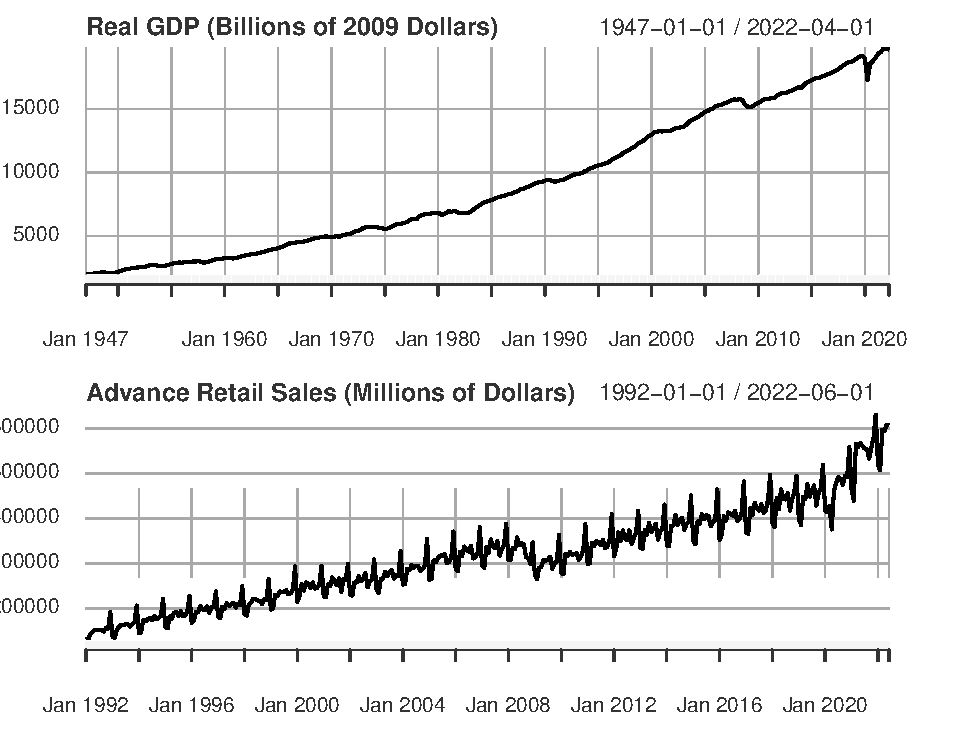
\includegraphics[width=0.8\linewidth]{bookdown-demo_files/figure-latex/ch1-figure1-1} 

}

\caption{Time Series at quarterly and monthly frequency}\label{fig:ch1-figure1}
\end{figure}

The first panel shows data for the real gross domestic product (GDP) for
the US in billions of 2012 dollars, measured at a quarterly frequency.
The second panel shows data for the advance retail sales (millions of
dollars), measured at monthly frequency.

Formally, we denote a time series variable by \(y_t\), where
\(t=0,1,2,..,T\) is the observation index. For example, at \(t=10\) we
get the tenth observation of this time series, \(y_{10}\).

\hypertarget{serial-correlation}{%
\section{Serial Correlation}\label{serial-correlation}}

Serial correlation (or auto correlation) refers to the tendency of
observations of a time series being correlated over time. It is a
measure of the temporal dynamics of a time series and addresses the
following question: what is the effect of past realizations of a time
series on the current period value? Formally,

\begin{equation}
\rho(s)=Cor(y_t, y_{t-s}) =\frac{   Cov(y_t,y_{t-s})}{\sqrt{\sigma^2_{y_t} \times \sigma^2_{y_{t-s}}}}
\label{eq:sercor}
\end{equation}

where \(Cov(y_t,y_{t-s})= E(y_t-\mu_{y_t})(y_{t-s}-\mu_{y_{t-s}})\) and
\(\sigma^2_{y_t}=E(y_t-\mu_{y_t})^2\)

Here, \(\rho(s)\) is the serial correlation of order \(s\). For example,
\(s=1\) implies \emph{first order} serial correlation between \(y_t\)
and \(y_{t-1}\), \(s=2\) implies \emph{second order} serial correlation
between \(y_t\) and \(y_{t-2}\), and so on.

Note that often we use historical data to forecast. If there is no
serial correlation, then past can offer no guidance for the present and
future. In that sense, presence of serial correlation of some order is
the first condition for being able to forecast a time series using its
historical realizations.

Now, we can either have positive or negative serial correlation in data.
Figure \ref{fig:ch1-figure2} plots two time series with positive and
negative serial correlation, respectively.

\begin{figure}

{\centering 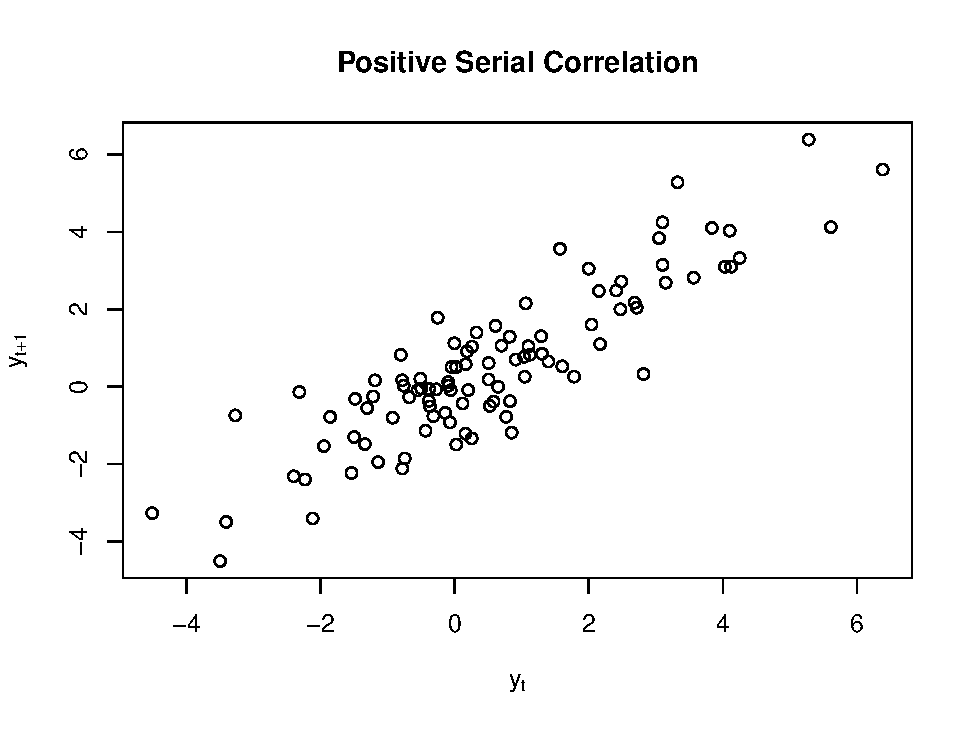
\includegraphics[width=0.8\linewidth]{bookdown-demo_files/figure-latex/ch1-figure2-1} 

}

\caption{Serial Correlation}\label{fig:ch1-figure21}
\end{figure}
\begin{figure}

{\centering 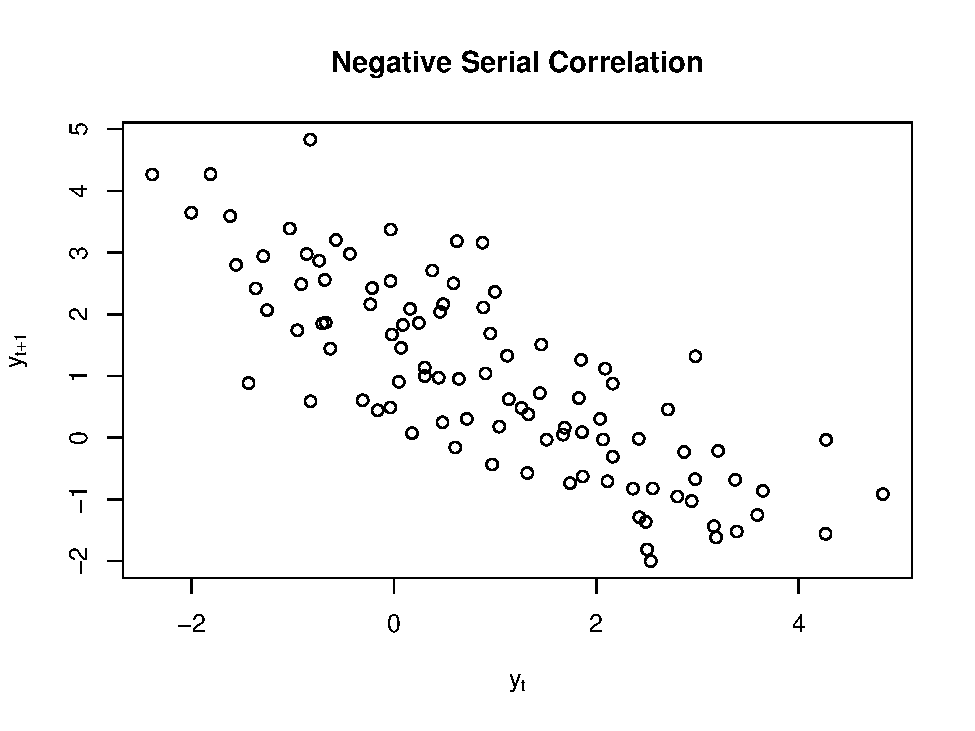
\includegraphics[width=0.8\linewidth]{bookdown-demo_files/figure-latex/ch1-figure2-2} 

}

\caption{Serial Correlation}\label{fig:ch1-figure22}
\end{figure}

\hypertarget{testing-for-serial-correlion}{%
\section{Testing for Serial
Correlion}\label{testing-for-serial-correlion}}

We can use a Lagrange-Multiplier (LM) test for detecting serial
correlation. This test is also known as \emph{Breuch-Godfrey} test. I
will use the linear regression model to explain this test. Consider the
following regression model: \begin{equation}
y_t=\beta_0 + \beta_1 X_{1t}+\epsilon_t
\end{equation}

Consider the following model for serial correlation of order \emph{p}
for the error term: \begin{equation}
\epsilon_t=\rho_1 \epsilon_{t-1}+\rho_2 \epsilon_{t-2}+...+ \rho_p \epsilon_{t-p}+\nu_t
\label{eq:bg}
\end{equation}

Then we are interested in the following test:

\[H_0=\rho_1=\rho_2=...=\rho_p=0 \] \[H_A = Not \ H_0 \]

To implement this test, we estimate the BG regression model given by:
\begin{equation}
e_t=\alpha_0 + \alpha_1 X_{1t}+ \rho_1 e_{t-1}+\rho_2 e_{t-2}+...+ \rho_p e_{t-p}+\nu_t
\label{eq:bg1}
\end{equation}

where we replacr the error term with the OLS residuals (denoted by
\(e\)). The LM test statistic is given by:

\[ LM  = N\times R^2_{BG}  \sim \chi^2_p  \]

If the test statistic value is greater than the critical value then we
reject the null hypothesis.

\hypertarget{white-noise-process}{%
\section{White Noise Process}\label{white-noise-process}}

A time series is a \emph{white noise} process is it has zero mean,
constant and finite variance, and is serially uncorrelated. Formally,
\(y_t\) is a white noise process if:

\begin{enumerate}
\def\labelenumi{\arabic{enumi}.}
\tightlist
\item
  \(E(y_t)=0\)
\item
  \(Var(y_t)=\sigma^2_y\)
\item
  \(Cov(y_t,y_{t-s})= 0 \forall s\neq t\)
\end{enumerate}

We can compress the above definition as: \(y_t\sim WN(0,\sigma^2_y)\).
Often we assume that the unexplained part of a time series follows a
white noise process. Formally,

\begin{equation}
Time \ Series \ = \  Explained  \ + \ White \ Noise
\end{equation}

By definition we cannot forecast a white noise process. An important
diagnostics of model adequacy is to test whether the estimated residuals
are white noise (more on this later).

\hypertarget{important-elements-of-forecasting}{%
\section{Important Elements of
Forecasting}\label{important-elements-of-forecasting}}

\BeginKnitrBlock{definition}[Forecast]
\protect\hypertarget{def:d1}{}{\label{def:d1} \iffalse (Forecast) \fi{} }
\EndKnitrBlock{definition}

A \emph{forecast} is an \emph{informed} guess about the unknown future
value of a time series of interest. For example, what is the stock price
of Facebook next Monday?

There are three possible types of forecasts:

\begin{enumerate}
\def\labelenumi{\arabic{enumi}.}
\tightlist
\item
  \emph{Density Forecast}: we forecast the entire probability
  distribution of the possible future value of the time series of
  interest. Hence,
\end{enumerate}

\begin{equation}
F(a)=P[y_{t+1}\leq a]
\end{equation}

give us the probability that the 1-period ahead future value of
\(y_{t+1}\) will be less than or equal to \(a\). For example, the future
real GDP growth could be normally distributed with a mean of 1.3\% and a
standard deviation of 1.83\%. Figure \ref{fig:ch1-figure3} below plots
the density forecast for real GDP growth.

\begin{figure}

{\centering 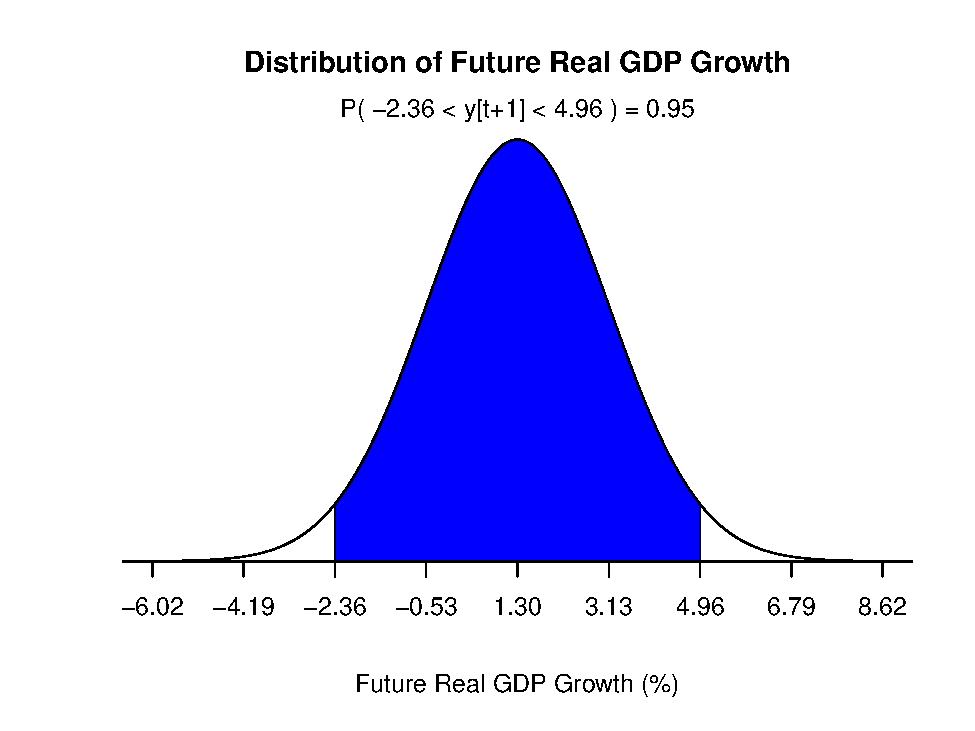
\includegraphics[width=0.8\linewidth]{bookdown-demo_files/figure-latex/ch1-figure3-1} 

}

\caption{Density Forecast for Future Real GDP Growth}\label{fig:ch1-figure3}
\end{figure}

\begin{enumerate}
\def\labelenumi{\arabic{enumi}.}
\setcounter{enumi}{1}
\item
  \emph{Point Forecast}: our forecast at each horizon is a single
  number. Often we use the expected value or mean as the point forecast.
  For example, the point forecast for the 1-period ahead real GDP growth
  can be the mean of the probability distribution of the future real GDP
  growth: \begin{equation}
  f_{t,1}=1.3%
  \end{equation}
\item
  \emph{Interval Forecast}: our forecast at each horizon is a range
  which is obtained by adding \emph{margin of errors} to the point
  forecast. With some probability we expect our future value to fall
  withing this range. For example, the 95\% interval forecast for the
  next period real GDP growth is (-2.36\%,4.96\%). Hence, with 95\%
  confidence we expect next period GDP to fall between -2.36\% and
  4.96\%.
\end{enumerate}

\BeginKnitrBlock{definition}[Forecast Horizon]
\protect\hypertarget{def:d2}{}{\label{def:d2} \iffalse (Forecast Horizon)
\fi{} }
\EndKnitrBlock{definition}

\emph{Forecast Horizon} is the number of periods into the future for
which we forecast a time series. We will denote it by \(h\). Hence, for
\(h=1\), we are looking at 1-period ahead forecast, for \(h=2\) we are
looking at 2-period ahead forecast and so on.

Formally, for a given time series \(y_t\), the h-period ahead unknown
value is denoted by \(y_{t+h}\). The forecast of this value is denoted
\(f_{t,h}\).

\begin{figure}

{\centering 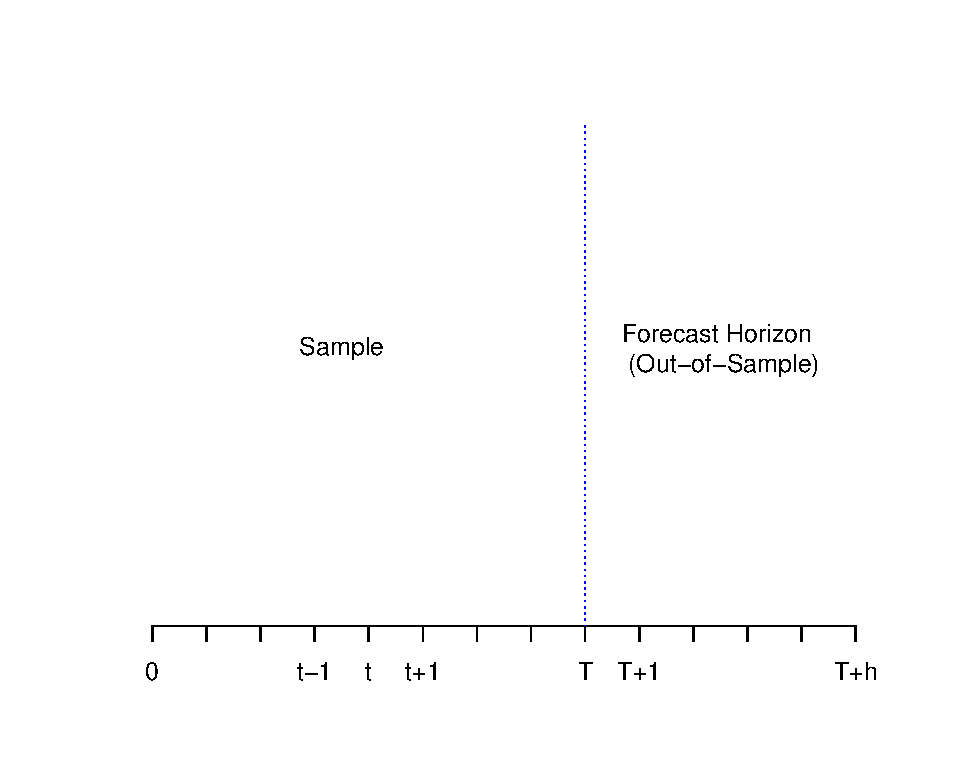
\includegraphics[width=0.8\linewidth]{bookdown-demo_files/figure-latex/ch1-figure4-1} 

}

\caption{Forecast Horizon}\label{fig:ch1-figure4}
\end{figure}

\BeginKnitrBlock{definition}[Forecast Error]
\protect\hypertarget{def:d3}{}{\label{def:d3} \iffalse (Forecast Error)
\fi{} }
\EndKnitrBlock{definition}

A \emph{forecast error} is the difference between the realization of the
future value and the previously made forecast. Formally, the
\(h\)-period ahead forecast error is given by:

\begin{equation}
e_{t,h}=y_{t+h}-f_{t,h}
\end{equation}

Hence, for every horizon, we will have a forecast and a corresponding
forecast error. These errors can be negative (indicating over
prediction) or positive (indicating under prediction).

\BeginKnitrBlock{definition}[Information Set]
\protect\hypertarget{def:d4}{}{\label{def:d4} \iffalse (Information Set)
\fi{} }
\EndKnitrBlock{definition}

Forecasts are based on \emph{information} available at the time of
making the forecast. \emph{Information Set} contains all the relevant
information about the time series we would like to forecast. We denote
the set of information available at time \(T\) by \(\Omega_T\). There
are two types of information sets:

\begin{enumerate}
\def\labelenumi{\arabic{enumi}.}
\item
  Univariate Information set: Only includes historical data on the time
  series of interest: \begin{equation}
  \Omega_T=\{y_T, y_{T-1}, y_{T-2}, ...., y_1\}
  \end{equation}
\item
  Multivariate Information set: Includes historical data on the time
  series of interest as well as any other variable(s) of interest. For
  example, suppose we have one more variable \(x\) that is relevant for
  forecasting \(y\). Then: \begin{equation}
  \Omega_T=\{y_T, x_T, y_{T-1}, x_{T-1}, y_{T-2},x_{T-2}. ...., y_1, x_1\}
  \end{equation}
\end{enumerate}

\hypertarget{loss-function-and-optimal-forecast}{%
\section{Loss Function and Optimal
Forecast}\label{loss-function-and-optimal-forecast}}

Think of a forecast as a solution to an \emph{optimization} problem.
When forecasts are wrong, the person making the forecast will suffer
some \emph{loss}. This loss will be a function of the magnitude as well
as the sign of the \emph{forecast error}. Hence, we can think of an
\emph{optimal forecast} as a solution to a minimization problem where
the forecaster is minimizing the loss from the forecast error.

\BeginKnitrBlock{definition}[Loss Function]
\protect\hypertarget{def:d5}{}{\label{def:d5} \iffalse (Loss Function) \fi{}
}
\EndKnitrBlock{definition}

A \emph{loss} function is a mapping between forecast errors and their
associated losses. Formally, we denote the h-period ahead loss function
by \(L(e_{t,h})\). For a function to be used as a loss function, three
properties must be satisfied:

\begin{enumerate}
\def\labelenumi{\arabic{enumi}.}
\tightlist
\item
  \(L(0)=0\)
\item
  \(\frac{dL}{de}>0\)
\item
  \(L(e)\) is a continuous function.
\end{enumerate}

Two types of loss functions are:

\begin{itemize}
\tightlist
\item
  Symmetric Loss Function: both positive and negative forecast errors
  lead to same loss. See Figure \ref{fig:ch1-figure5}. A commonly used
  loss function is \emph{quadratic loss function} given by:
\end{itemize}

\begin{equation}
L(e_{t,h})=e_{t,h}^2 = (y_{t+h}-f{t,h})^2
\end{equation}

\begin{figure}

{\centering 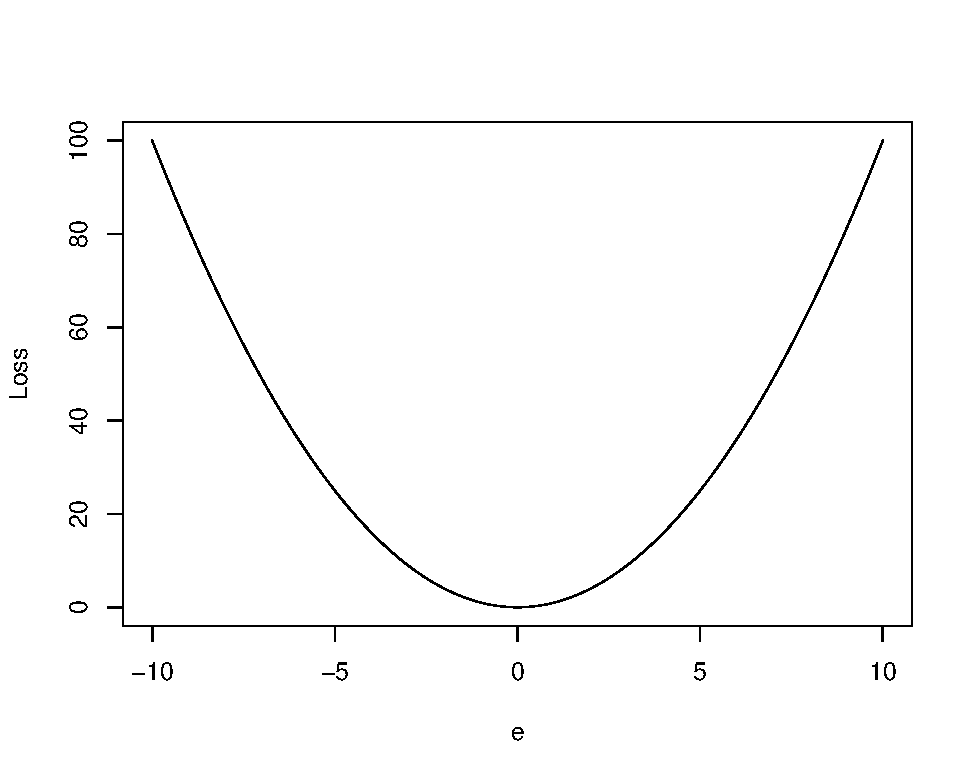
\includegraphics[width=0.8\linewidth]{bookdown-demo_files/figure-latex/ch1-figure5-1} 

}

\caption{Quadratic Loss Functions}\label{fig:ch1-figure5}
\end{figure}

\begin{itemize}
\tightlist
\item
  Asymmetric Loss Function: loss depends on the sign of the forecast
  error. For example, it could be that positive errors produce greater
  loss when compared to negative errors. See the function below and
  Figure \ref{fig:ch1-figure6} that attaches a higher loss to positive
  errors:
\end{itemize}

\begin{equation}
L(e_{t,h})=e_{t,h}^2+4 \times e_{t,h}
\end{equation}

\begin{figure}

{\centering 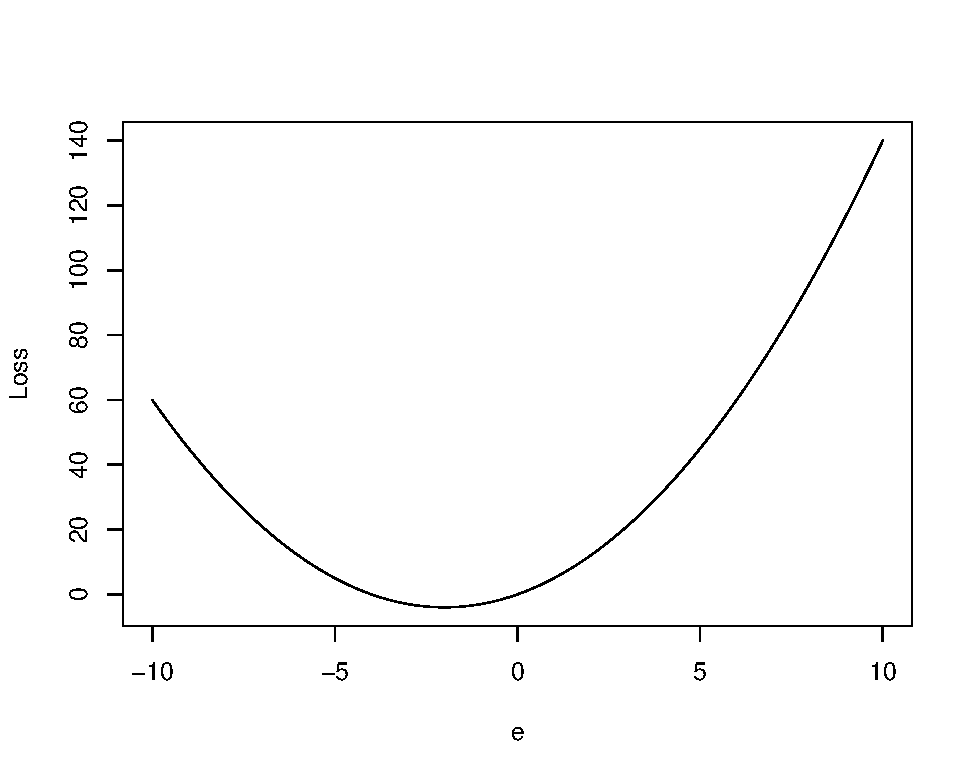
\includegraphics[width=0.8\linewidth]{bookdown-demo_files/figure-latex/ch1-figure6-1} 

}

\caption{Asymmetric Loss Function}\label{fig:ch1-figure6}
\end{figure}

Once we have chosen our loss function, the optimal forecast can be
obtained by minimizing the expected loss function.

\BeginKnitrBlock{definition}[Optimal Forecast]
\protect\hypertarget{def:d6}{}{\label{def:d6} \iffalse (Optimal Forecast)
\fi{} }
\EndKnitrBlock{definition}

An \emph{optimal forecast} minimizes the expected loss from the
forecast, given the information available at the time. Mathematically,
we denote it by \(f^*_{t,h}\) and it solves the following minimization
problem: \begin{equation}
min_{f_{t,h}} E(L(e_{t,h})|\Omega_t)
\end{equation}

In theory we can assume any functional form for the loss function and
that will lead to a different \emph{optimal forecast}. An important
result that follows from a specific functional form is stated as Theorem
1.1.

\BeginKnitrBlock{theorem}
\protect\hypertarget{thm:unnamed-chunk-2}{}{\label{thm:unnamed-chunk-2} }If
the loss function is quadtratic then the optimal forecast is the
conditional mean of the time series of interest. Formally, if
\(L(e_{t,h})=e_{t,h}^2\) then, \begin{equation}
f^*_{t,h}=E(y_{t+h}|\Omega_t)
\end{equation}
\EndKnitrBlock{theorem}

Note that \(E(e_{t,h}^2)\) is known as \emph{mean squared errors (MSE)}.
Hence, the expected loss from a quadratic loss function is the same as
the MSE. In this course, we assume that the forecaster faces a quadratic
loss function and hence based on Theorem 1.1, we will learn different
models for estimating the conditional mean of the future value of the
time series of interest, i.e., \(E(y_{t+h}|\Omega_t)\).

\hypertarget{regression-based-forecasting}{%
\chapter{Regression-based
Forecasting}\label{regression-based-forecasting}}

One way to compute the conditional expectation is the linear regression
model. Here, our information set contains data on all relevant
explanatory variables available at the time of forecast, i.e,

\begin{equation}
\Omega_t={X_{1t}, X_{2t},...X_{Kt}}
\end{equation}

Hence, we get the following equality:

\begin{equation}
E(y_t|\Omega_t)=E(y_{t}|X_{1t}, X_{2t}, X_{3t},...,X_{Kt})
\end{equation}

The right hand side of the above equation is the multiple regression
model of the form: \begin{equation}
 y_{t}=\beta_0+\beta_1 X_{1t}+\beta_2 X_{2t}+..+\beta_K X_{Kt}+\epsilon_t
 \end{equation}

We can easily estimate the above model using Ordinary Least Squares
(OLS) and compute the \emph{predicted value} of \(y\): \begin{equation}
    \widehat{y}_t = \widehat{\beta_0} +\widehat{\beta_1} X_{1t} +\widehat{\beta_2} X_{2t}+...+ \widehat{\beta_k} X_{Kt}
  \end{equation}

The above equation can be used to compute the optimal forecast. Suppose,
we are interested in computed the \(h\) period ahead forecast for \(y\).
Then, using the above equation we get: \begin{equation}
        \widehat{y}_{t+h} =  \widehat{\beta_0} +\widehat{\beta_1} X_{1t+h} +\widehat{\beta_2} X_{2t+h}+...+ \widehat{\beta_k} X_{Kt+h}
    \end{equation}

\hypertarget{scenario-analysis-and-conditional-forecasts}{%
\section{Scenario Analysis and Conditional
Forecasts}\label{scenario-analysis-and-conditional-forecasts}}

One way to use a regression model to produce forecasts is called
\emph{scenario analysis} where we produce a different forecast for the
dependent under each possible scenario about the future values of the
independent variables. For example, what will be the forecast for
inflation if the Federal Reserve Bank raises the interest rate? Would
our forecast differ depending on the size of the increase in the
interest rate?

\hypertarget{unconditional-forecasts}{%
\section{Unconditional Forecasts}\label{unconditional-forecasts}}

An alternative is to separately forecast each independent variable and
then compute the forecast for the dependent variable. Yet another
alternative is to use lagged variables as independent variables.
Depending on the number of lags, we can forecast that much ahead into
future (see Distributed Lag Section for details).

\hypertarget{some-practical-issues}{%
\section{Some practical issues}\label{some-practical-issues}}

\begin{enumerate}
\def\labelenumi{\arabic{enumi}.}
\item
  To forecast the dependent variable we first need to compute a forecast
  for the independent variable. Errors in this step induce errors later.
\item
  \emph{Spurious regression}: It is quite possible to find a strong
  linear relationship between two completely unrelated variables over
  time if they share a common time trend.
\item
  \emph{Model Uncertainty}: We do not know the true functional form for
  the regression model and hence our estimated model is only a proxy for
  the true model.
\item
  \emph{Parameter Uncertainty}: This kind of forecast uses regression
  coefficients that are computed using a fixed sample. Over time with
  new data, there will be changes in these coefficients.
\end{enumerate}

\hypertarget{distributed-lag-regression-models}{%
\section{Distributed Lag Regression
Models}\label{distributed-lag-regression-models}}

Consider the following simple regression model:

\begin{equation}
y_t= \beta_0 +\beta_1 x_t + \epsilon_t
\end{equation}

Here, if want to forecast \(y_{t+1}\) then we must either consider
different scenarios for \(x_{t+1}\) or independently forecast
\(x_{t+1}\) first, and then use it to compute forecast for \(y_{t+1}\).
An alternative is to estimate the following lagged regression model:

\begin{equation}
y_t= \beta_0 +\beta_1 x_{t-1} + \epsilon_t
\end{equation}

Note that by estimating the above model we get the following predicted
value equation for \(t+1\):

\begin{equation}
\widehat{y_{t+1}}=\widehat{\beta_0}+\widehat{\beta_1}x_{t}
\end{equation}

Hence, we can easily produce 1-period ahead forecast from this model. In
order to produce forecast farther into future we would need to add more
lags of the independent variable to the model. A generalized model of
this kind is called \emph{distributed lag model} and is given by:
\begin{equation}
y_t= \beta_0 +\sum_{s=1}^p\beta_s x_{t-s} + \epsilon_t
\end{equation}

The number of lags to include can be determined using some kind of
goodness of fit measure.

\hypertarget{dynamic-effect-of-x-on-y}{%
\subsection{Dynamic Effect of X on Y}\label{dynamic-effect-of-x-on-y}}

A very useful benefit of estimating a distributed lag model is that it
allows us to measure how changes in \(x\) in the current period can
impact the dependent variable over time. Consider a simple distributed
lag model with two lags: \begin{equation}
y_t=\beta_0 + \beta_1 x_{t-1} + \beta_2 x_{t-2} +\epsilon_t
\end{equation}

In this model the lag structure implies that any change in \(x\) will
persist for two periods in terms of its effect on \(y\). In fact we now
have to consider the \emph{dynamic} effect of \(x\) on \(y\). Formally,
there are two types of effects:

\begin{enumerate}
\def\labelenumi{\arabic{enumi}.}
\tightlist
\item
  \emph{dynamic effect} of \(x\) on \(y\) given by:
  \[ \frac{\partial y_{t+s}}{\partial x_t} \quad s=0,1,2,... \]
\end{enumerate}

In our example, the sequence of dynamic effects are: \begin{equation}
\frac{\partial y_{t}}{\partial x_t}  =0; \ \frac{\partial y_{t+1}}{\partial x_t}=\beta_1; \ \frac{\partial y_{t+2}}{\partial x_t}=\beta_2; \ \frac{\partial y_{t+s}}{\partial x_t}=0 \ \forall \ s>2 
\end{equation}

\begin{enumerate}
\def\labelenumi{\arabic{enumi}.}
\setcounter{enumi}{1}
\tightlist
\item
  \emph{long run effect} of \(x\) on \(y\) given by: \begin{equation}
  \sum_{s=0}^p\frac{\partial y_{t+s}}{\partial x_t}   
  \end{equation}
\end{enumerate}

In our example, the long run effect is:

\[\beta_1+\beta_2\]

\hypertarget{model-selection-criterion}{%
\subsection{Model Selection Criterion}\label{model-selection-criterion}}

Most often we compare models that have different number of independent
variables. For example, in our application, in order to select the
number of lags for output and capital stock, we will essentially compare
models with different number of independent variables. In such cases we
must account for the trade-off between goodness of fit and degrees of
freedom. Increasing the number of independent variables will:

\begin{enumerate}
\def\labelenumi{\arabic{enumi}.}
\item
  lower the MSE and hence leads to better fit.
\item
  lowers the degrees of freedom
\end{enumerate}

Two commonly used measures based on MSE incorporate this trade-off:

\begin{enumerate}
\def\labelenumi{\arabic{enumi}.}
\tightlist
\item
  Akaike Information Criterion (AIC):
  \[ AIC= MSE \times e^{\frac{2k}{T}} \]
\end{enumerate}

where \(k\) is the number of estimated parameters, \(T\) is the sample
size. Then, \(K/T\) is the number of parameters estimated per
observation and \(e^{\frac{2k}{T}}\) is the \emph{penalty factor}
imposed on adding more variables to the model. As we increase \(k\),
this penalty factor will increase exponentially for a given value of
\(T\).

\begin{enumerate}
\def\labelenumi{\arabic{enumi}.}
\setcounter{enumi}{1}
\tightlist
\item
  Bayesian Information Criterion (BIC):
\end{enumerate}

\[ BIC= MSE \times T^{\frac{k}{T}} \]

Lower values of either AIC or BIC indicates greater accuracy. So we
select a model with lower value of either of these two criteria. Note
that the penalty imposed by BIC is harsher and hence it will typically
select a more parsimonious model (Figure \ref{fig:ch2-figure1}).

\begin{figure}

{\centering 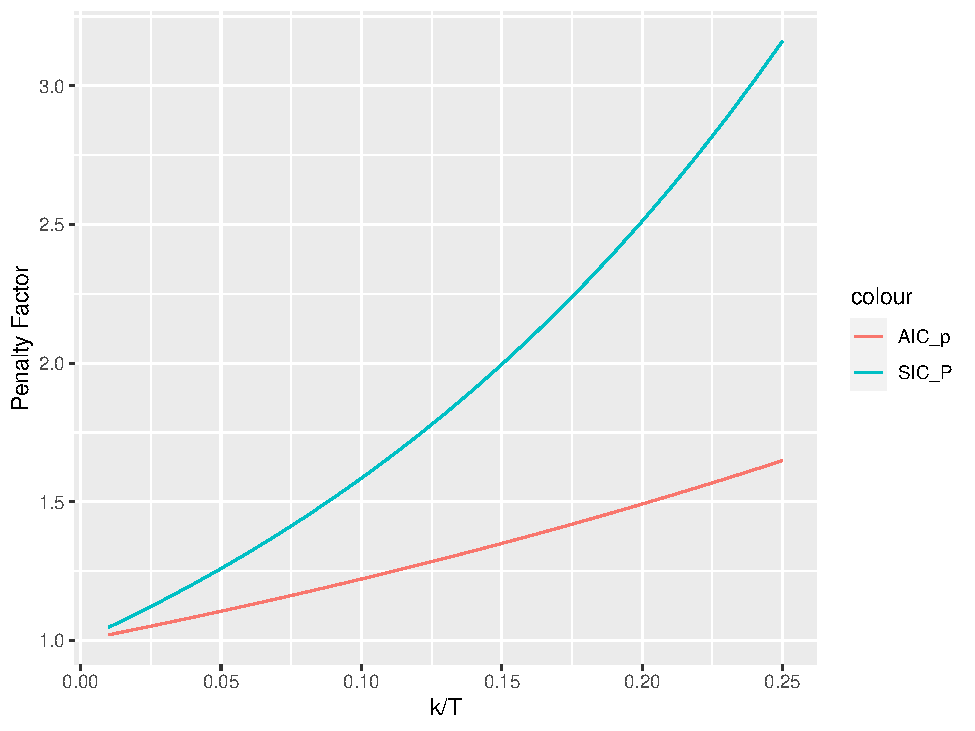
\includegraphics[width=0.8\linewidth]{bookdown-demo_files/figure-latex/ch2-figure1-1} 

}

\caption{Penalty Factor of AIC and BIC}\label{fig:ch2-figure1}
\end{figure}

\hypertarget{application-a-model-of-investment-expenditure}{%
\section{Application: A Model of Investment
Expenditure}\label{application-a-model-of-investment-expenditure}}

\hypertarget{a-multiple-regression-model-of-invesment-expenditure}{%
\subsection{A Multiple Regression Model of Invesment
Expenditure}\label{a-multiple-regression-model-of-invesment-expenditure}}

Suppose have annual data on private investment, private sector output,
and capital stock. Our model specification is given by: \begin{equation}
y_t= \beta_0 + \beta_1 x_{1t}+ \beta_2 x_{2t}+\epsilon_t
\end{equation}

We can estimate the above model using OLS and then conduct
scenario-based forecasting. For ease of interpretation, we will convert
all variables in natural logarithms.

Table \ref{tab:ch2-table1} below presents the estimated coefficients of
our regression model. Higher output and capital stock leads to greater
investment expenditure.

\begin{table}

\caption{\label{tab:ch2-table1}A Multiple Regression Model of Investment Expenditure}
\centering
\begin{tabular}[t]{lcccc}
\toprule
  & Estimated Coefficients & Std. Error & t-ratio & p-value\\
\midrule
(Intercept) & -4.8421855 & 0.9623332 & -5.031714 & 0.0000044\\
x1 & 0.9987751 & 0.2418282 & 4.130102 & 0.0001104\\
x2 & 0.4204833 & 0.3643054 & 1.154205 & 0.2528456\\
\bottomrule
\end{tabular}
\end{table}

Next, we forecast of investment expenditure under three different
scenarios:

\begin{enumerate}
\def\labelenumi{\arabic{enumi}.}
\item
  For next 3 years, both output and capital stock remain at the average
  of last 3 years.
\item
  For next 3 years, both output and capital stock remain at 1\% above
  the average of last 3 years.
\item
  For next 3 years, both output and capital stock remain at 1\% below
  the average of last 3 years.
\end{enumerate}

Figure \ref{fig:ch2-figure2} below present our investment expenditure
outlook under these 3 scenarios.

\begin{figure}

{\centering 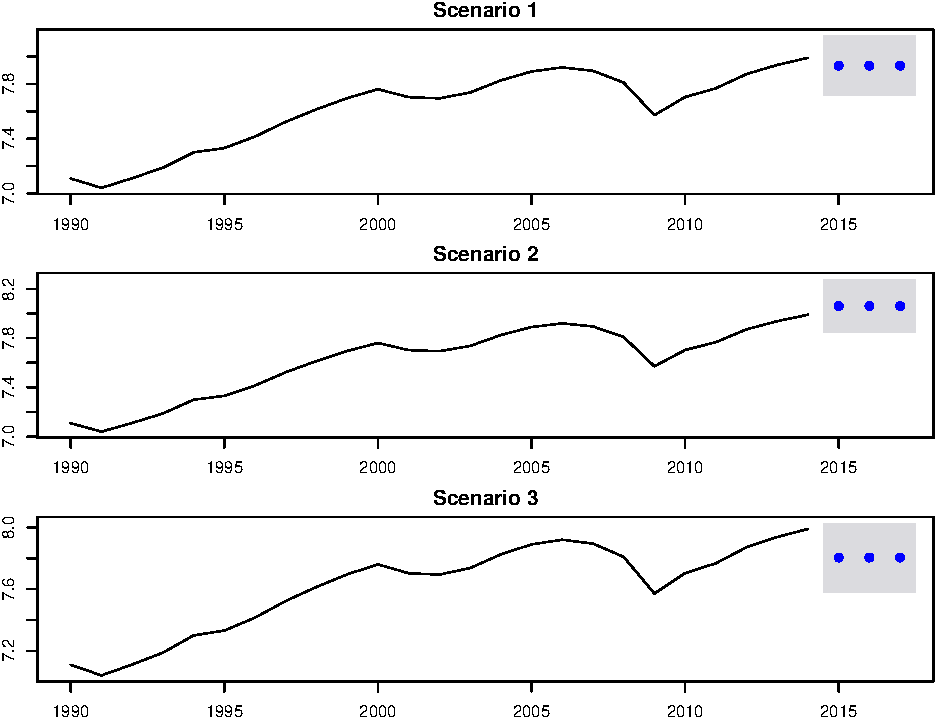
\includegraphics[width=0.8\linewidth]{bookdown-demo_files/figure-latex/ch2-figure2-1} 

}

\caption{Investment outlook for next 3 years}\label{fig:ch2-figure2}
\end{figure}

\hypertarget{a-distributed-lag-model-of-investment-expenditure}{%
\subsection{A Distributed Lag Model of Investment
Expenditure}\label{a-distributed-lag-model-of-investment-expenditure}}

In this application we will estimate a distributed lag model for
investment expenditure. The idea here is that it takes time for
investment to respond to output and capital stock changes. The model
specification we want to estimate is:

\begin{equation}
y_t= \beta_0 + \sum_{i=1}^p\beta_i x_{1t-i}+\sum_{i=1}^p\alpha_i x_{2t-i}+\epsilon_t
\end{equation}

where \(y\) denotes real investment expenditure of the private sector,
\(x_1\) denotes output of the private sector, and \(x_2\) denotes
capital stock of the private sector.

We estimate our model by first selecting the optimal lag order for each
independent variable, and selecting the one with lowest value for
AIC/BIC. From @\ref(tab:ch2-table2) we find that the lowest BIC occurs
at lag=2. Hence, we estimate a model with two lags for each independent
variable in our model.

\begin{table}

\caption{\label{tab:ch2-table2}Optimal Order of the lags}
\centering
\begin{tabular}[t]{ccc}
\toprule
Lag & AIC & BIC\\
\midrule
1 & -98.42469 & -89.72714\\
2 & -127.36043 & -114.31411\\
3 & -129.95355 & -112.55845\\
4 & -127.49885 & -105.75498\\
\bottomrule
\end{tabular}
\end{table}

Hence, our final model is given by: \begin{equation}
y_t= \beta_0 + \sum_{i=1}^2\beta_i x_{1t-i}+\sum_{i=1}^2\alpha_i x_{2t-i}
\end{equation}

The results of our estimation are presented below in Table
\ref{tab:ch2-table3}

\begin{table}

\caption{\label{tab:ch2-table3}Distributed Lag Model of Investment Expenditure}
\centering
\begin{tabular}[t]{lcccc}
\toprule
  & Estimated Coefficients & Std. Error & t-ratio & p-value\\
\midrule
(Intercept) & -6.541336 & 0.8300877 & -7.880295 & 0.0000000\\
L(x1, 1:2)1 & 10.932987 & 1.9354346 & 5.648854 & 0.0000005\\
L(x1, 1:2)2 & -9.769632 & 1.9286226 & -5.065601 & 0.0000044\\
L(x2, 1:2)1 & 2.545657 & 0.7735580 & 3.290842 & 0.0017028\\
L(x2, 1:2)2 & -2.189088 & 0.7904689 & -2.769354 & 0.0075309\\
\bottomrule
\end{tabular}
\end{table}

\begin{enumerate}
\def\labelenumi{\arabic{enumi}.}
\item
  Using our estimated model we can easily compute the dynamic effect as
  well as the long run effect of each independent variable on the
  dependent variable.
\item
  Given the lag structure of our estimated model, we can also produce
  forecasts for \(y_{t+1}\) by computing the following equation:
\end{enumerate}

\begin{equation}
f_{t,1}=\widehat{y_{t+1}}=\hat{\beta_0}+\hat{\beta_1}x_{1t} + \hat{\beta_2}x_{1t-1}+ \hat{\alpha_1}x_{2t}+\hat{\alpha_2}x_{2t-1}
\end{equation}

\hypertarget{components-of-a-time-series}{%
\chapter{Components of a Time
Series}\label{components-of-a-time-series}}

A given time series can have four possible components:

\begin{enumerate}
\def\labelenumi{\arabic{enumi}.}
\item
  Trend: denoted by \(B_t\) captures the long run behavior of the time
  series of interest.
\item
  Season: denoted by \(S_t\) are \emph{periodic} fluctuations over
  \emph{seasons}. The period of the season is fixed and known. For
  example, rise in non-durable sales during Christmas.
\item
  Cycle: denoted by \(C_t\) are \emph{non-periodic} are fluctuations in
  that they occur regularly but over periods that are not fixed in
  duration.
\item
  Irregular: denoted by \(\epsilon_t\) are random fluctuations,
  typically modeled as a white noise process.
\end{enumerate}

\hypertarget{decomposing-a-time-series}{%
\section{Decomposing a time series}\label{decomposing-a-time-series}}

We can decompose any given time series into its components. There are
two ways to accomplish this:

\begin{enumerate}
\def\labelenumi{\arabic{enumi}.}
\item
  Additive Decomposition: Here it is assumed that all four components
  are added to obtain the underlying timer series: \begin{equation}
  y_t= B_t+S_t+C_t +\epsilon_t
  \end{equation}
\item
  Multiplicative Decomposition: Here it is assumed that all four
  components are multiplied to obtain the underlying timer series:
  \begin{equation}
  y_t= B_t \times S_t \times C_t \times \epsilon_t
  \end{equation}
\end{enumerate}

Note that using properties of logarithms, multiplicative decomposition
is the same as additive decomposition in log terms: \begin{equation}
log(y_t)= log(B_t) + log(S_t) + log(C_t) + log(\epsilon_t)
\end{equation}

Most statistical software can implement these decomposition using data
on a time series variable as input. Typically they combine cyclical
component with irregular component and provide a three-way
decomposition. In Figure \ref{fig:ch3-figure1} I use R to decompose real
GDP for the US into its components.

\begin{figure}

{\centering 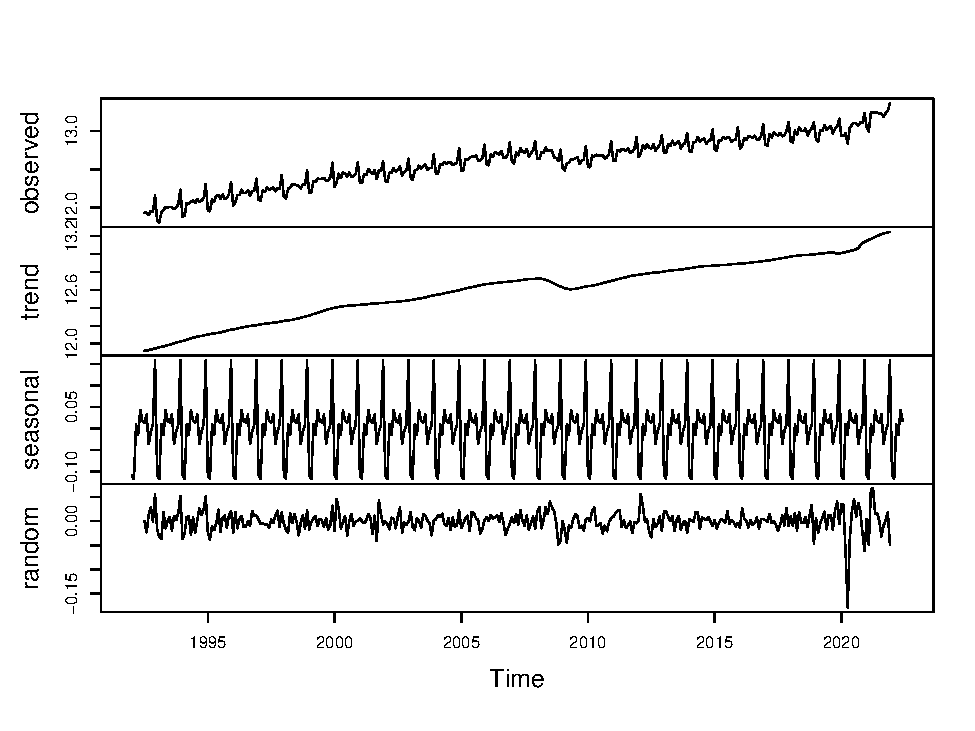
\includegraphics[width=0.8\linewidth]{bookdown-demo_files/figure-latex/ch3-figure1-1} 

}

\caption{Additive Decomposition of Retail Sales}\label{fig:ch3-figure1}
\end{figure}

\hypertarget{uses-of-decomposition-of-a-time-series}{%
\section{Uses of Decomposition of a time
series}\label{uses-of-decomposition-of-a-time-series}}

The usefulness of decomposing a time series depends on our objective.

\begin{enumerate}
\def\labelenumi{\arabic{enumi}.}
\item
  It may be of interest to study each component separately or to simply
  improve our understanding of the temporal dynamics of a time series of
  interest. Decomposing it into different components is the first step
  towards achieving that goal.
\item
  We can also use the decomposition to filter out components that we are
  not interested in studying. If for example we are only interested in
  modeling the cyclical component of the time series, then we can assume
  some kind decomposition, additive or multiplicative, and filter out
  the trend and seasonal component. For example, assuming additive
  decomposition, the filtered time series is given by: \begin{equation}
  Filtered \ y_t= y_t-B_t-S_t
  \end{equation}
\end{enumerate}

We can then proceed to model the cyclical component using the filtered
data.

\hypertarget{smoothing-methods}{%
\chapter{Smoothing Methods}\label{smoothing-methods}}

One way to approach forecasting is to \emph{average} out the
fluctuations in the underlying time series to produce a \emph{smoothed}
data which can be extrapolated to produce forecasts. These smoothing
methods are essentially \emph{model-free} and may not even produce
\emph{optimal forecasts}. Depending on the method used one can
accommodate seasonal as well as trend components of the underlying time
series.

\hypertarget{moving-average-method}{%
\section{Moving Average Method}\label{moving-average-method}}

We compute an average of most recent data values for the time series and
use it as a forecast for the next period.

An important parameter is the \emph{window} over which we take the
average. Let us denote this window by \(m\), then: \begin{equation}
    y^s_{t+1}=\frac{\sum \limits_{i=t-m+1}^{t}{y_i}}{m}
    \end{equation}

A larger value of \(m\) produces greater smoothing and most software
have a default value of this parameter which can be changed if needed.

\hypertarget{simple-exponential-smoothing}{%
\section{Simple Exponential
Smoothing}\label{simple-exponential-smoothing}}

In the moving average method, all observations received same weight.
However, it is reasonable to argue that more recent observations may
have a greater influence than those in the remote past. In this method,
the weight attached to past observations exponentially decay over time.
Here is the algorithm for computing the smoothed data and its forecast:

\begin{enumerate}
\def\labelenumi{\arabic{enumi}.}
\item
  Initialize at t=1: \[y_1^s=y_1\]
\item
  Update:
  \[y_{t}^{s}= \alpha y_t + (1-\alpha)y_{t-1}^{s}  \quad for \ t=2,3,...T\]
\end{enumerate}

3: h-period ahead forecast: \[f_{T,h}= y_T^s\]

Here the h-period ahead forecast is:

\emph{Exercise: Can you show that \(y_{t}^{s}\) is a is the weighted
moving average of all past observations? Use backward substitution
method.}

Here \(\alpha \in (0,1)\) is the smoothing parameter, with smaller value
indicating greater smoothing.

\hypertarget{holt-winters-smoothing}{%
\section{Holt-Winters Smoothing}\label{holt-winters-smoothing}}

We add trend component to the simple exponential smoothing. In step 2
the equation we use to update the smoothed data is given by:

\begin{align}
    y_{t}^{s}= \alpha y_t + (1-\alpha)(y_{t-1}^{s}+B_{t-1}) \\ \nonumber
    B_t = \beta (y_t^s -y_{t-1}^s) + (1-\beta) B_{t-1}
 \end{align}

We now have an additional parameter \(\beta\) that is the trend
parameter. Here the h-period ahead forecast is:

\begin{align}
  f_{T,h} = y_T^s + h\times B_T
  \end{align}

\hypertarget{holt-winters-smoothing-with-seasonality}{%
\section{Holt-Winters Smoothing with
Seasonality}\label{holt-winters-smoothing-with-seasonality}}

We now add seasonal component along with trend. Assuming multiplicative
seasonality with period \(n\):

\begin{align}
    y_{t}^{s}= \alpha \frac{y_t}{S_{t-n}} + (1-\alpha)(y_{t-1}^{s}+B_{t-1})\\
    B_t = \beta (y_t^s -y_{t-1}^s) + (1-\beta) B_{t-1}\\
    S_t = \gamma\frac{y_t}{y_t^s}+(1-\gamma)S_{t-n}
  \end{align}

The h-period ahead forecast is given by:

\begin{equation}
    f_{T,h}= (y_T^s + h\times B_T) \times S_{T+h-n}
   \end{equation}

\hypertarget{application}{%
\section{Application}\label{application}}

We use R to implement a 12-period ahead forecast for retail sales for
the U.S. The data is at monthly frequency from 1959 through 2015. We use
natural logs of the data and compute smoothed series using each of the
three methods. The resulting forecasts are plotted in Figure
\ref{fig:ch4-figure1}.

\begin{figure}

{\centering 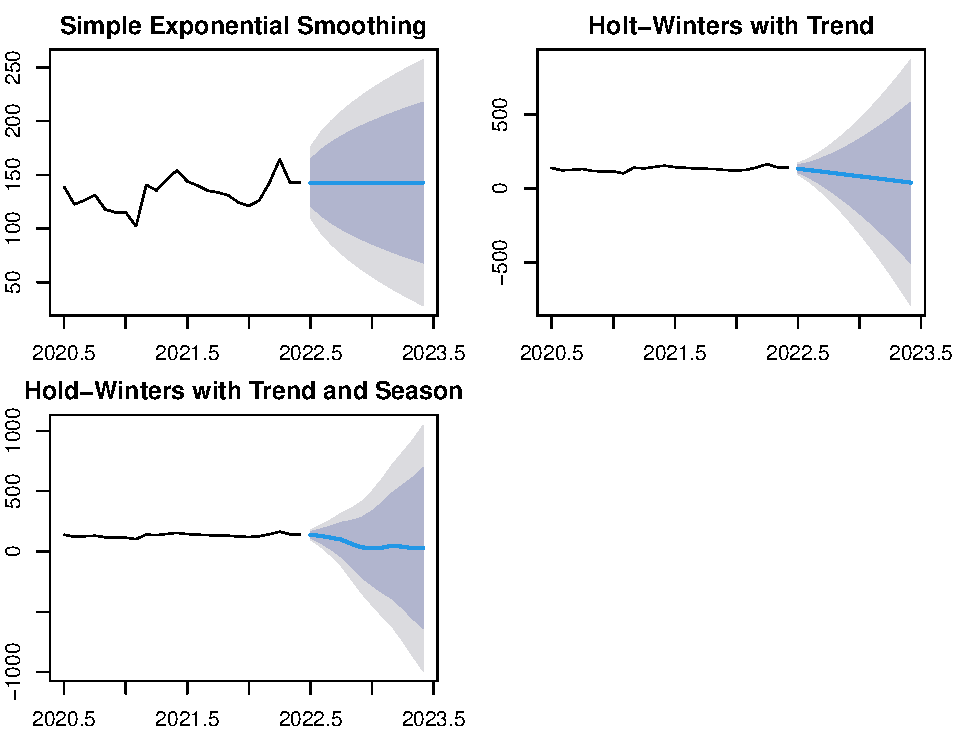
\includegraphics[width=0.8\linewidth]{bookdown-demo_files/figure-latex/ch4-figure1-1} 

}

\caption{Forecast of Housing Starts: Three Smoothing Methods}\label{fig:ch4-figure1}
\end{figure}

\hypertarget{modeling-trend-and-seasonal-components}{%
\chapter{Modeling Trend and Seasonal
Components}\label{modeling-trend-and-seasonal-components}}

\hypertarget{trend-estimation}{%
\section{Trend Estimation}\label{trend-estimation}}

An important component of a time series is \emph{trend} that captures
the long run evolution of the variable of interest. There are two types
of trends:

\begin{enumerate}
\def\labelenumi{\arabic{enumi}.}
\item
  Deterministic Trend: the underlying trend component is a \emph{known}
  function of time with \emph{unknown} parameters.
\item
  Stochastic Trend: the trend component is random.
\end{enumerate}

In this note we will focus on estimating and forecasting deterministic
trend models. We will come back to stochastic trend later when we talk
about stationarity property of a time series.

\hypertarget{parametrizing-a-deterministic-trend}{%
\subsection{Parametrizing a deterministic
trend}\label{parametrizing-a-deterministic-trend}}

Whether or not there is deterministic trend in the data can be typically
gleaned by simply plotting the time series over time. For example,
Figure @ref(fig: ch5-figure1) below plots real GDP for the US at
quarterly frequency. We can observe a positive time trend with real GDP
increasing with time. In this section we will learn to \emph{fit} a
function that captures this relationship accurately.

\begin{figure}

{\centering 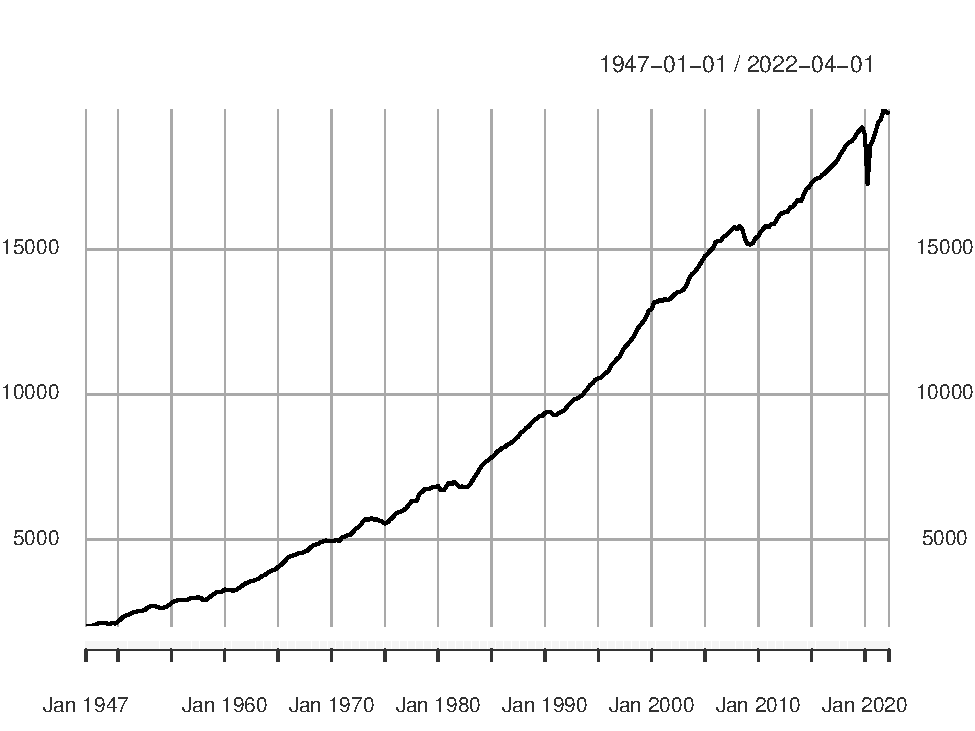
\includegraphics[width=0.8\linewidth]{bookdown-demo_files/figure-latex/ch5-figure1-1} 

}

\caption{Real GDP (2012 Chained Billions of Dollars)}\label{fig:ch5-figure1}
\end{figure}

\emph{Note: The variable time is denoted by \(t\) and it is artificially
created to take value of 1 for the first period, 2 for the second period
and so on.}

There are two commonly used functional forms for capturing a
deterministic trend:

\begin{enumerate}
\def\labelenumi{\arabic{enumi}.}
\tightlist
\item
  Polynomial Trend: We fit a polynomial of appropriate order to capture
  the time trend. For example, A. Linear trend: \begin{equation}
  y_t=\beta_0 +\beta_1 t +\epsilon_t
  \end{equation}
\end{enumerate}

B. Quadratic trend: \begin{equation}
y_t=\beta_0 +\beta_1 t + \beta_2 t^2 +\epsilon_t
\end{equation}

In general, we can fit a polynomial of order \(q\): \begin{equation}
y_t=\beta_0 + \sum_{i=1}^q \beta_i t^i +\epsilon_t
\end{equation}

We can estimate this model using the OLS. One of the key component here
is to determine the \emph{right} order of the polynomial. We can begin
with a large enough number for \(q\) and then select the appropriate
order using AIC or BIC criterion.

\begin{enumerate}
\def\labelenumi{\arabic{enumi}.}
\setcounter{enumi}{1}
\tightlist
\item
  Exponential or log-linear trend: In some cases we may want to use an
  exponential trend or equivalently a log-linear trend. \begin{align}
  y_t=e^(\beta_0 +\beta_1 t +\epsilon_t)\\
  equivalently\\
  log(y_t)=\beta_0 +\beta_1 t +\epsilon_t
  \end{align}
\end{enumerate}

Again we can estimate the above model using OLS.

\hypertarget{uses-of-the-deterministic-trend-model}{%
\subsection{Uses of the Deterministic Trend
Model}\label{uses-of-the-deterministic-trend-model}}

Once we have finalized our deterministic trend model i.e., either a
polynomial of a specific order or log-liner trend, we can use the
estimated model for the following two purposes:

\begin{enumerate}
\def\labelenumi{\arabic{enumi}.}
\item
  Detrending our data: Suppose we would like to eliminate trend from our
  data. The residual from our final trend model is the \emph{detrended}
  time series.
\item
  Forecasting: We can also forecast our time series based on the
  estimated trend. For example, suppose our final model is a quadratic
  trend. The predicted value is given by:
\end{enumerate}

\begin{equation}
\widehat{y_t}=\widehat{\beta_0}+\widehat{\beta_1} t + \widehat{\beta_2} t^2
\end{equation}

Then, the 1-period ahead forecast for \(y_{t+1}\) can be obtained by
solving: \begin{equation}
\widehat{y_{t+1}}=\widehat{\beta_0}+\widehat{\beta_1} (t+1) + \widehat{\beta_2} (t+1)^2
\end{equation}

\hypertarget{application-estimating-a-polynomial-trend-for-u.s.-real-gdp}{%
\subsection{Application: Estimating a polynomial trend for U.S. Real
GDP}\label{application-estimating-a-polynomial-trend-for-u.s.-real-gdp}}

We will now fit a polynomial trend to the US real GDP data that was
presented in Figure \ref{fig:figure10}. We first estimate polynomials of
different orders and select the optimal order determined by the lowest
possible AIC/BIC. Table \ref{tab:ch5-table1}. shows these statistics for
up to 4th order polynomial. We find that the lowest value occur at
\(q=4\).

\begin{table}

\caption{\label{tab:ch5-table1}Optimal Order of the Polynomial}
\centering
\begin{tabular}[t]{ccc}
\toprule
order & AIC & BIC\\
\midrule
1 & 4716.836 & 4727.794\\
2 & 4133.469 & 4148.079\\
3 & 4105.087 & 4123.350\\
4 & 4002.212 & 4024.127\\
\bottomrule
\end{tabular}
\end{table}

Hence, our final trend model is:

\begin{equation}
y_t=\beta_0 +\beta_1 t + \beta_2 t^2 + \beta_3 t^3 + \beta_4 t^4 +\epsilon_t
\end{equation}

The estimated trend model is presented in Table \ref{tab:ch5-table2}.

\begin{table}

\caption{\label{tab:ch5-table2}Regression Results}
\centering
\begin{tabular}[t]{lcccc}
\toprule
  & Estimate & Std. Error & t value & Pr(>|t|)\\
\midrule
(Intercept) & 1714.277 & 81.019 & 21.159 & 0\\
trend & 43.398 & 3.911 & 11.097 & 0\\
I(trend\textasciicircum{}2) & -0.344 & 0.055 & -6.194 & 0\\
I(trend\textasciicircum{}3) & 0.003 & 0.000 & 10.233 & 0\\
I(trend\textasciicircum{}4) & 0.000 & 0.000 & -11.160 & 0\\
\bottomrule
\end{tabular}
\end{table}

Using the estimated model, we can compute the detrended data as the
residual and also forecast \(y_t\). Figure \ref{fig:ch5-figure2} below
plots the detrended real GDP obtained as a residual from our trend
model.

\begin{figure}

{\centering 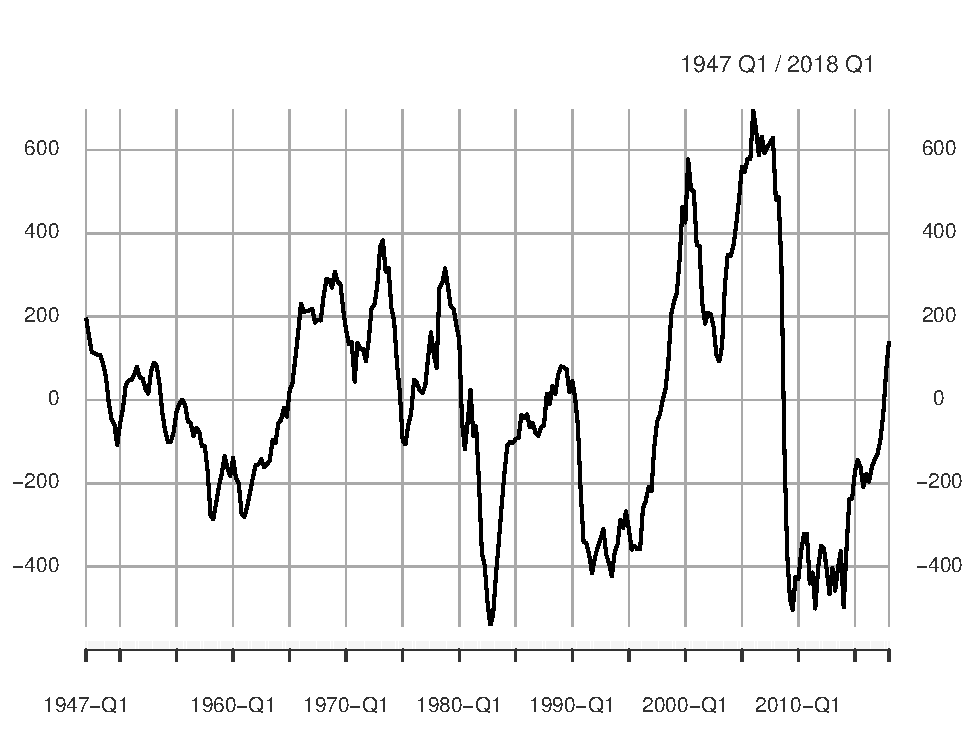
\includegraphics[width=0.8\linewidth]{bookdown-demo_files/figure-latex/ch5-figure2-1} 

}

\caption{Detrended Real GDP}\label{fig:ch5-figure2}
\end{figure}

Figure \ref{fig:ch5-figure3} shows the forecast of real GDP for next 8
quarters along with the 95\% confidence bands.

\begin{figure}

{\centering 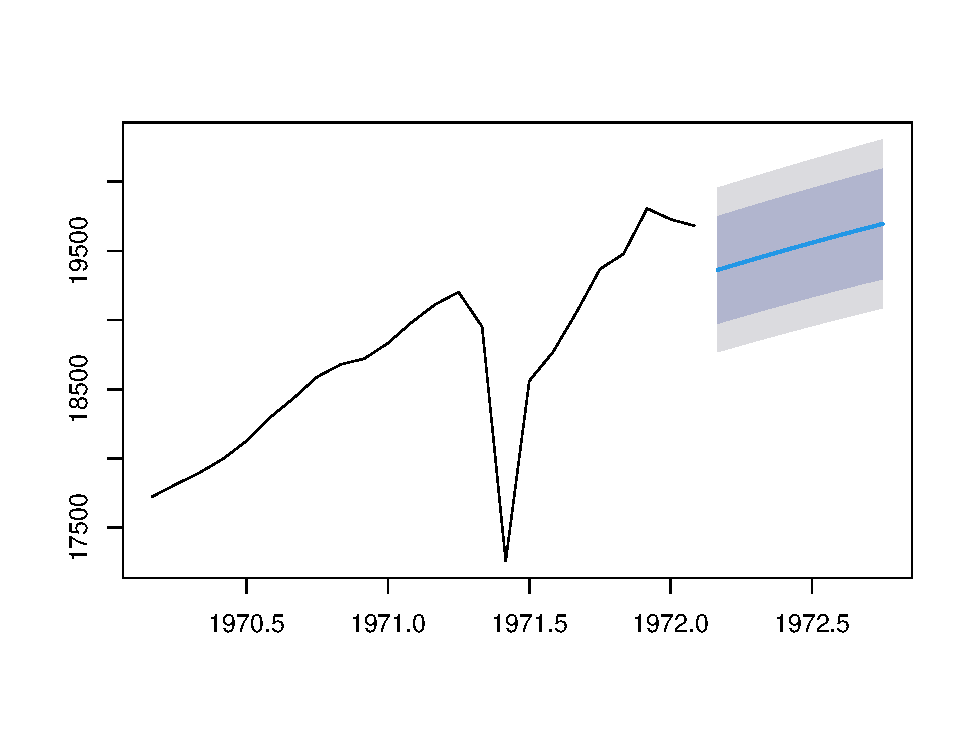
\includegraphics[width=0.8\linewidth]{bookdown-demo_files/figure-latex/ch5-figure3-1} 

}

\caption{Forecast of Real GDP}\label{fig:ch5-figure3}
\end{figure}

\hypertarget{seasonal-model}{%
\section{Seasonal Model}\label{seasonal-model}}

We now focus on the \emph{seasonal} component of a time series, i.e.,
that is periodic fluctuations that repeat themselves every season. For
example, increase in ice cream sales during summer season. Just like
trend component, such seasonal pattern could be \emph{deterministic} or
\emph{stochastic}. In this chapter we will focus on estimating
deterministic seasonal component.

In Figure \ref{fig:ch5-figure4} we plot housing starts in the U.S. The
data is at monthly frequency and we can see a clear seasonal pattern.
Housing starts seem to increase in spring and summer months. This is
followed by a decline in fall and winter months.

\begin{figure}

{\centering 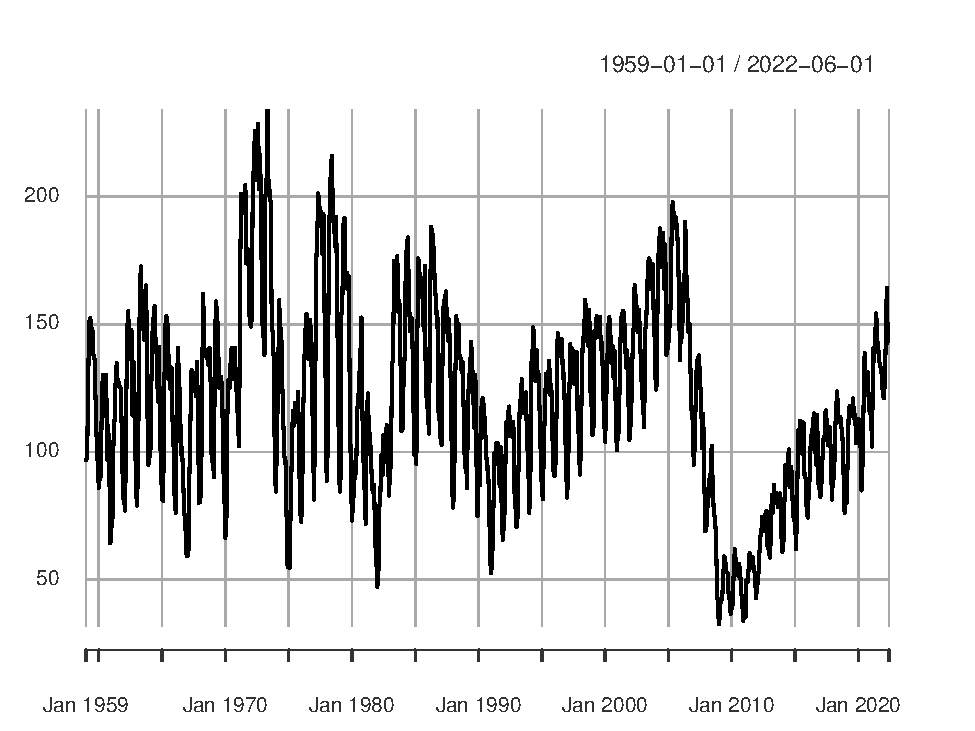
\includegraphics[width=0.8\linewidth]{bookdown-demo_files/figure-latex/ch5-figure4-1} 

}

\caption{Housing Starts in U.S.}\label{fig:ch5-figure4}
\end{figure}

One option to deal with seasonality is to either obtain seasonally
adjusted data from the source itself. Alternatively, we can use
decomposition method and appropriately filter out the seasonal
component. However, if our objective is to explicitly model the seasonal
component of a time series then we must work with non-seasonally
adjusted data.

\hypertarget{regression-model-with-seasonal-dummy-variables}{%
\subsection{Regression Model with Seasonal Dummy
Variables}\label{regression-model-with-seasonal-dummy-variables}}

One way to account for seasonal patterns in data is to add dummy
variables for season. To avoid perfect multicollinearity, is there are
\(s\) seasons, we can include \(s-1\) dummy variables. For example, for
quarterly data, \(s=4\) and hence we need \(s-1=3\) dummy variables in
our regression model. Formally, for quarterly data, the seasonal
regression model is given by:

\begin{equation}
y_t= \beta_0 + \beta_1 D_{1t}+ \beta_2 D_{2t} + \beta_3 D_{3t} + \epsilon_t
\end{equation}

In the above regression model, \(D_1,D_2,\) and \(D_3\) are dummy
variables that capture first three quarters of the year. For example,
\(D_1=1\) for the first quarter and \(D_1=0\) otherwise. Similarly,
\(D_2=1\) for the second quarter and \(D_2=0\) otherwise. In this
example, we use the fourth quarter as the \emph{base group}.

The above model can be estimated using OLS. Again, we can use the
residual from our estimated model as a measure of \emph{deseasonlized}
data. We can also forecast the dependent variable based on the seasonal
component only.

\hypertarget{application-seasonal-model-of-housing-starts}{%
\subsection{Application: Seasonal Model of Housing
Starts}\label{application-seasonal-model-of-housing-starts}}

We now estimate a seasonal regression model for the housing starts data
presented in Figure \ref{fig:ch5-figure4}. The data is at monthly
frequency which implies we can have 12 possible seasons and hence would
need 11 dummy variables in our regression model. Formally, we use
January as the base group and include dummy variables for the last 11
months of the year:

\begin{equation}
y_t=\beta_0 + \sum_{i=2}^{12}\beta_i D_{it} + \epsilon_t
\end{equation}

Table \ref{tab:ch5-table3} presents the estimation results for this
exercise. In Figure \ref{fig:ch5-figure5} we plot the forecast of
housing starts for next 12 months using our estimated model, along with
95\% confidence bands.

\begin{table}

\caption{\label{tab:ch5-table3}Regression Results}
\centering
\begin{tabular}[t]{lcccc}
\toprule
  & Estimate & Std. Error & t value & Pr(>|t|)\\
\midrule
(Intercept) & 84.422 & 9.852 & 8.569 & 0.000\\
season2 & 2.283 & 13.933 & 0.164 & 0.870\\
season3 & 19.133 & 13.933 & 1.373 & 0.171\\
season4 & 28.350 & 13.933 & 2.035 & 0.043\\
season5 & 34.061 & 13.933 & 2.445 & 0.015\\
\addlinespace
season6 & 35.562 & 13.749 & 2.587 & 0.010\\
season7 & 33.422 & 13.933 & 2.399 & 0.017\\
season8 & 27.794 & 13.933 & 1.995 & 0.047\\
season9 & 26.139 & 13.933 & 1.876 & 0.062\\
season10 & 25.622 & 13.933 & 1.839 & 0.067\\
\addlinespace
season11 & 10.489 & 13.933 & 0.753 & 0.452\\
season12 & 0.639 & 13.933 & 0.046 & 0.963\\
\bottomrule
\end{tabular}
\end{table}

\begin{figure}

{\centering 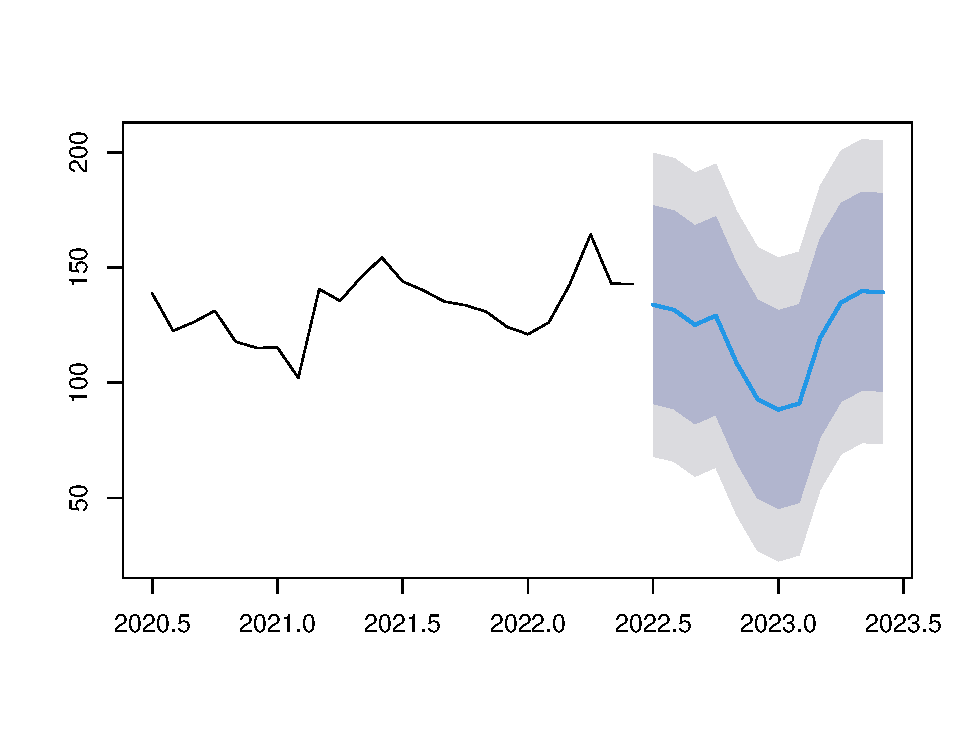
\includegraphics[width=0.8\linewidth]{bookdown-demo_files/figure-latex/ch5-figure5-1} 

}

\caption{Forecast of Housing Starts}\label{fig:ch5-figure5}
\end{figure}

\hypertarget{autoregressive-moving-average-arma-model}{%
\chapter{Autoregressive Moving Average (ARMA)
Model}\label{autoregressive-moving-average-arma-model}}

In this chapter we will focus on the cyclical component of a time series
and hence focus on data that either has no trend and seasonal
components, or data that is filtered to eliminate any trend and
seasonality. One of the most commonly used method to model cyclicality
is the \emph{Autogressive Moving Average (ARMA)}. We first learn some
new concepts that will help us in understanding the properties of this
model.

\hypertarget{covariance-stationary-time-series}{%
\section{Covariance Stationary Time
Series}\label{covariance-stationary-time-series}}

\BeginKnitrBlock{definition}[Covariance Stationary Time Series]
\protect\hypertarget{def:d7}{}{\label{def:d7} \iffalse (Covariance
Stationary Time Series) \fi{} }
\EndKnitrBlock{definition}

A time series \(\{y_t\}\) is said to be a \emph{covariance stationary
process} if:

\begin{enumerate}
\def\labelenumi{\arabic{enumi}.}
\tightlist
\item
  \(E(y_t)=\mu_x \quad \forall \quad t\)
\item
  \(Var(y_t)=\sigma_x^2 \quad \forall \quad t\)
\item
  \(Cov(y_t,y_{t-s})=\gamma(s) \quad \forall \quad s\neq t\)
\end{enumerate}

One way to think about stationarity is \emph{mean-reversion}, i.e, the
tendency of a time series to return to its \emph{long-run} unconditional
mean following a shock (or a series of shock). Figure
@\ref(fig:ch6-figure1) below shows this property graphically.

\begin{figure}

{\centering 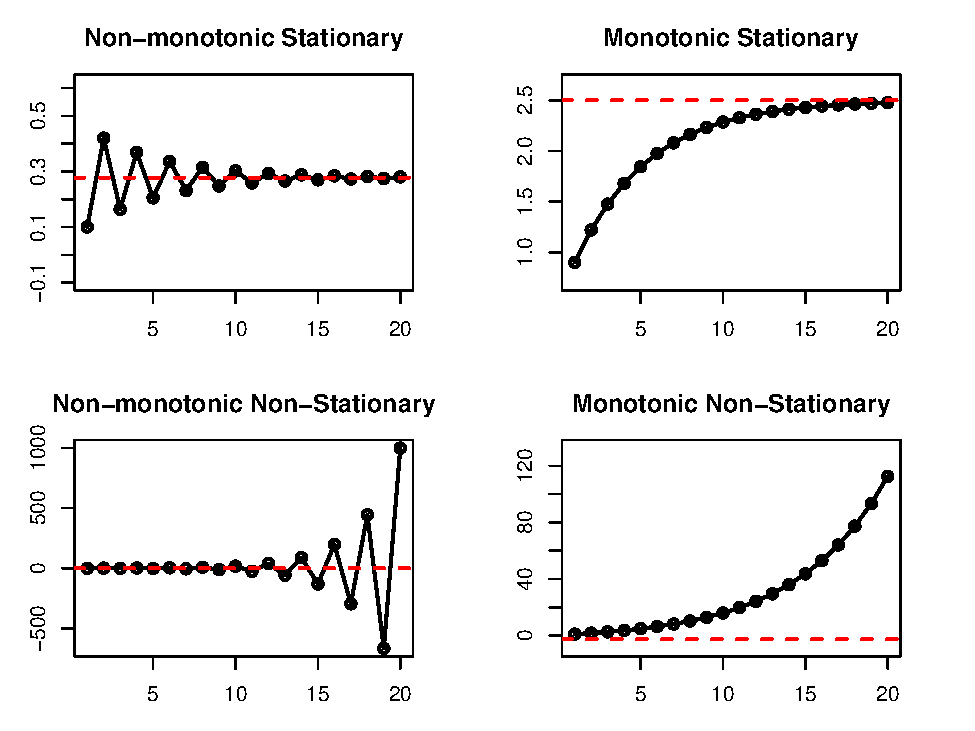
\includegraphics[width=0.8\linewidth]{bookdown-demo_files/figure-latex/ch6-figure1-1} 

}

\caption{Reversion to mean}\label{fig:ch6-figure1}
\end{figure}

\begin{figure}

{\centering 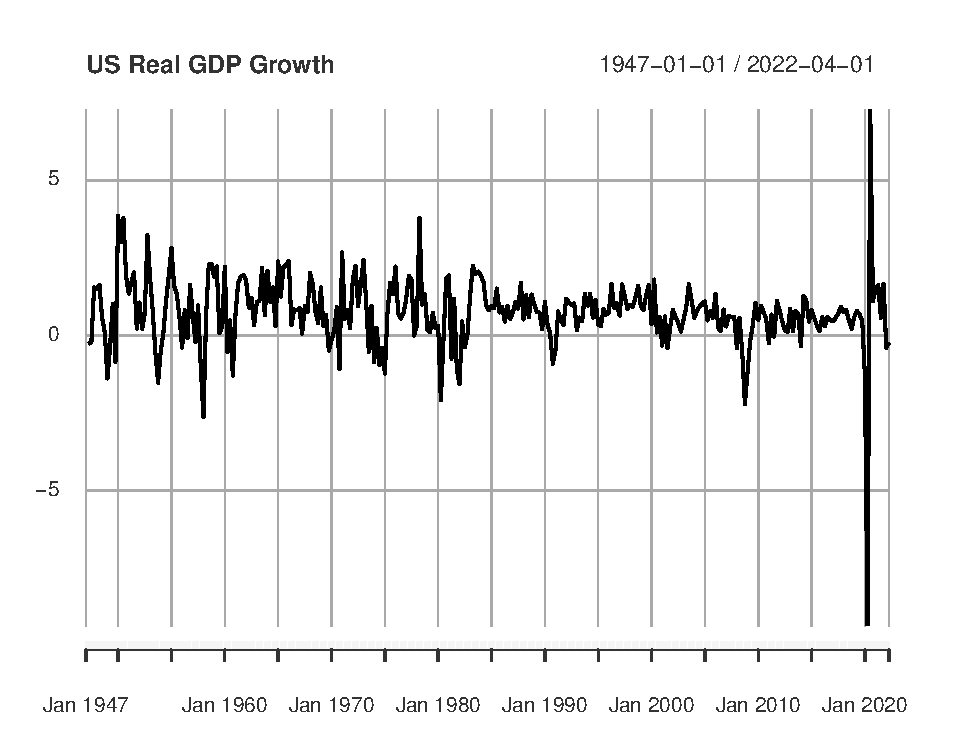
\includegraphics[width=0.8\linewidth]{bookdown-demo_files/figure-latex/ch6-figure2-1} 

}

\caption{Reversion to mean in practice}\label{fig:ch6-figure2}
\end{figure}

In practice however, you will not be able to visualize a mean-reverting
stationary process this clearly. For example, in Figure
\ref{fig:ch6-figure2} we plot real GDP growth for the U.S. which is a
stationary process with a mean of 0.7\%. In this chapter we will only
consider stationary time series data. Later on we will learn how to work
with non-stationary data.

\hypertarget{correlation-over-time}{%
\section{Correlation over time}\label{correlation-over-time}}

In order to forecast into future, we need information available in the
present to correlate with the future value of the variable of interest.
In other words, we need some serial correlation in our data which can be
utilized to generate forecasts. In general, for a time series,
\(\{y_t\}\), \begin{align}
    Cor(y_t,y_{t-s})=\frac{ Cov(y_t,y_{t-s})}{\sqrt{\sigma^2_{y_t} \times \sigma^2_{y_{t-s}}}}
        \end{align} where
\(Cov(y_t,y_{t-s})= E(y_t-\mu_{y_t})(y_{t-s}-\mu_{y_{t-s}})\) and
\(\sigma^2_{y_t}=E(y_t-\mu_{y_t})^2\)

\BeginKnitrBlock{definition}[Auto Correlation Function (ACF)]
\protect\hypertarget{def:d8}{}{\label{def:d8} \iffalse (Auto Correlation
Function (ACF)) \fi{} }
\EndKnitrBlock{definition}

An \emph{ACF} plots the correlation of a time series with its own past
values over time. For a stationary time series, using the three
conditions we get: \begin{align}
    ACF(s) \ or \ \rho(s)=\frac{\gamma(s)}{\gamma(0)}
    \end{align}

Hence, non-zero values of the ACF indicates presences of serial
correlation in the data. Figure \ref{fig:ch6-figure3} shows the ACF for
a stationary time series with positive serial correlation.

\begin{figure}

{\centering 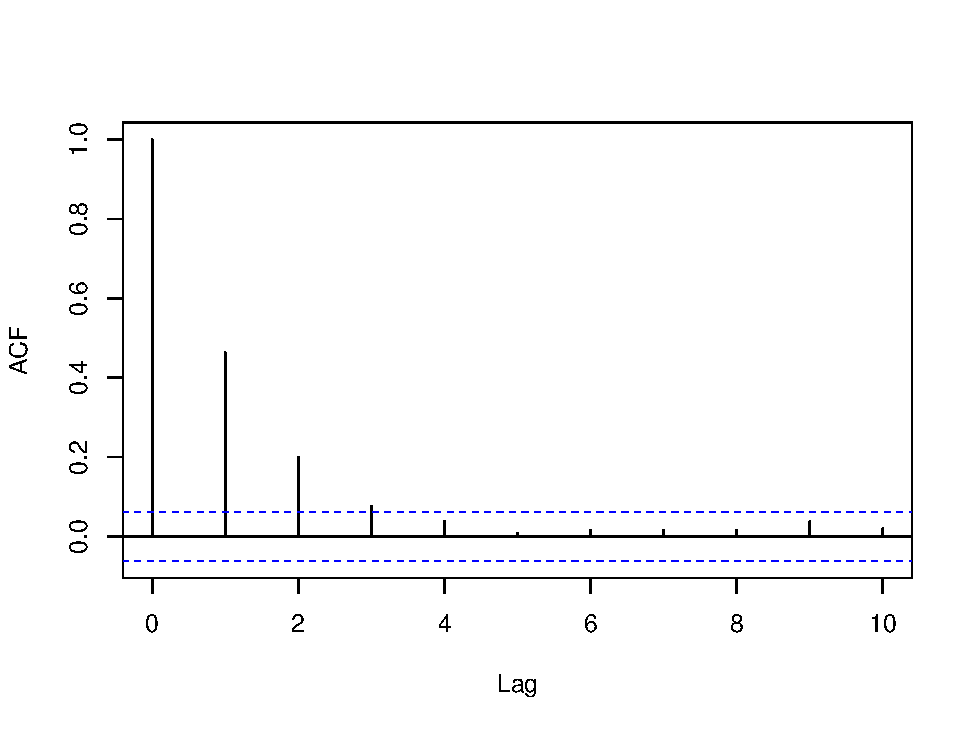
\includegraphics[width=0.8\linewidth]{bookdown-demo_files/figure-latex/ch6-figure3-1} 

}

\caption{ACF for a Stationary Time Series}\label{fig:ch6-figure3}
\end{figure}

\BeginKnitrBlock{definition}[Partial Auto Correlation Function (PACF)]
\protect\hypertarget{def:d9}{}{\label{def:d9} \iffalse (Partial Auto
Correlation Function (PACF)) \fi{} }
\EndKnitrBlock{definition}

The \emph{partial autocorrelation function (PACF)} for a stationary time
series \(y_t\) at lag \(s\) is the direct correlation between \(y_t\)
and \(y_{t-s}\), after filtering out the linear influence of \$
y\_\{t-1\},\ldots,y\_\{t-s-1\}\$ on \(y_t\). Figure
\ref{fig:ch6-figure4} below shows the PACF for a stationary time series
where only one lag directly affects the time series in the current
period.

\begin{figure}

{\centering 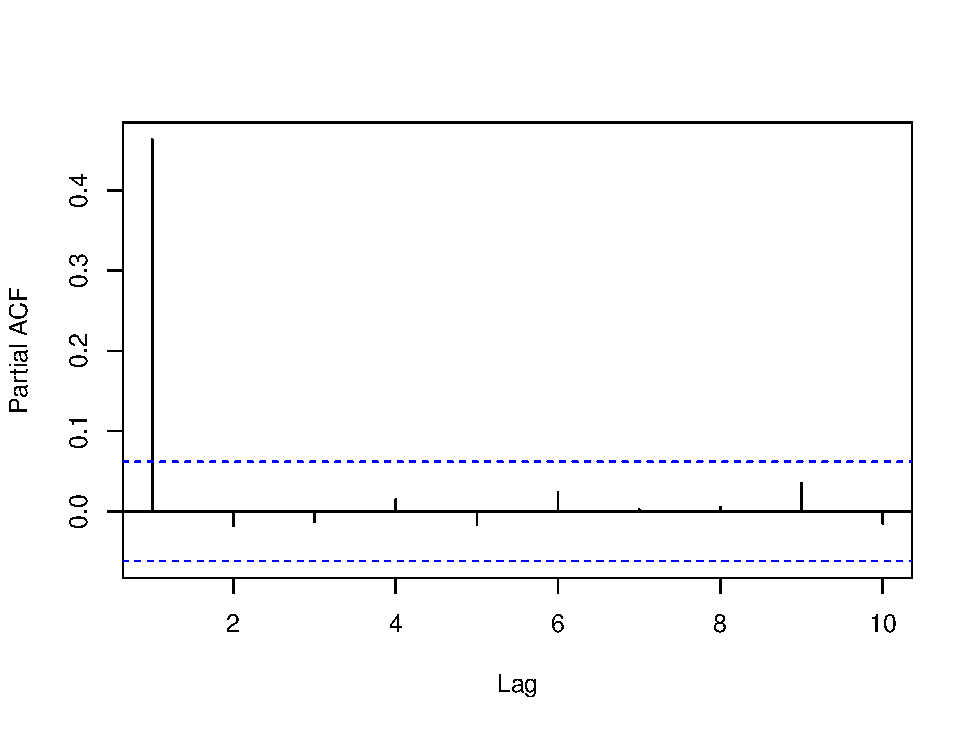
\includegraphics[width=0.8\linewidth]{bookdown-demo_files/figure-latex/ch6-figure4-1} 

}

\caption{PACF for a Stationary Time Series}\label{fig:ch6-figure4}
\end{figure}

\hypertarget{autoregressive-ar-model}{%
\section{Autoregressive (AR) Model}\label{autoregressive-ar-model}}

A \emph{stationary}time series \(\{x_t\}\) can be modeled as an AR(p)
process: \begin{equation}
 y_t = \phi_0 +\phi_1 y_{t-1} + \phi_2 y_{t-2} + ...... + \phi_p y_{t-p}+\epsilon_t
 \end{equation}

\hypertarget{moving-average-ma-model}{%
\section{Moving Average (MA) Model}\label{moving-average-ma-model}}

A \emph{stationary} time series \(\{y_t\}\) can be modeled as an MA(q)
process: \begin{equation}
  y_t = \theta_0 + \epsilon_t + \theta_1 \epsilon_{t-1} + \theta_2 \epsilon_{t-2} + ...... + \theta_q \epsilon_{t-q}
    \end{equation}

\hypertarget{armap-q}{%
\section{ARMA(p, q)\}}\label{armap-q}}

An ARMA model simply combines both AR and MA components to model the
dynamics of a time series. Formula,

\begin{equation}
   y_t = \phi_0 +\phi_1 x_{t-1} + \phi_2 y_{t-2} + ...... + \phi_p y_{t-p}+\epsilon_t + \theta_1 \epsilon_{t-1} + \theta_2 \epsilon_{t-2} + ...... + \theta_q \epsilon_{t-q}
   \end{equation}

\bibliography{book.bib,packages.bib}


\end{document}
